\documentclass[11pt, oneside]{article}   	% use "amsart" instead of "article" for AMSLaTeX format
\usepackage{geometry}                		% See geometry.pdf to learn the layout options. There are lots.
\geometry{letterpaper}                   		% ... or a4paper or a5paper or ... 
%\geometry{landscape}                		% Activate for rotated page geometry
%\usepackage[parfill]{parskip}    		% Activate to begin paragraphs with an empty line rather than an indent
\usepackage{graphicx}				% Use pdf, png, jpg, or eps§ with pdflatex; use eps in DVI mode
								% TeX will automatically convert eps --> pdf in pdflatex		
\usepackage{amssymb}

\usepackage{listings} 
\usepackage{color}
\definecolor{dkgreen}{rgb}{0,0.6,0}

\lstset{
   breaklines=true,                                     % line wrapping on
   language=SQL,
   %frame=ltrb,
   framesep=5pt,
   basicstyle=\normalsize,
   %keywordstyle=\ttfamily\color{OliveGreen},
   %identifierstyle=\ttfamily\color{CadetBlue}\bfseries,
   commentstyle=\color{dkgreen},
   stringstyle=\ttfamily,
   showstringspaces=ture
}

% Add your keywords here, and have this in a separate file
% and include it in your preamble
\lstset{emph={ 
    DATETIME, REFERENCES
    },emphstyle={\textbf}
}


\title{CS 660: Project Assignment \#1}
\author{Bowen Zhang (U881677028) \\Yiwen Gu (U58170649)}
\date{}							% Activate to display a given date or no date

\begin{document}
\maketitle
\section{The ER-Diagram}				
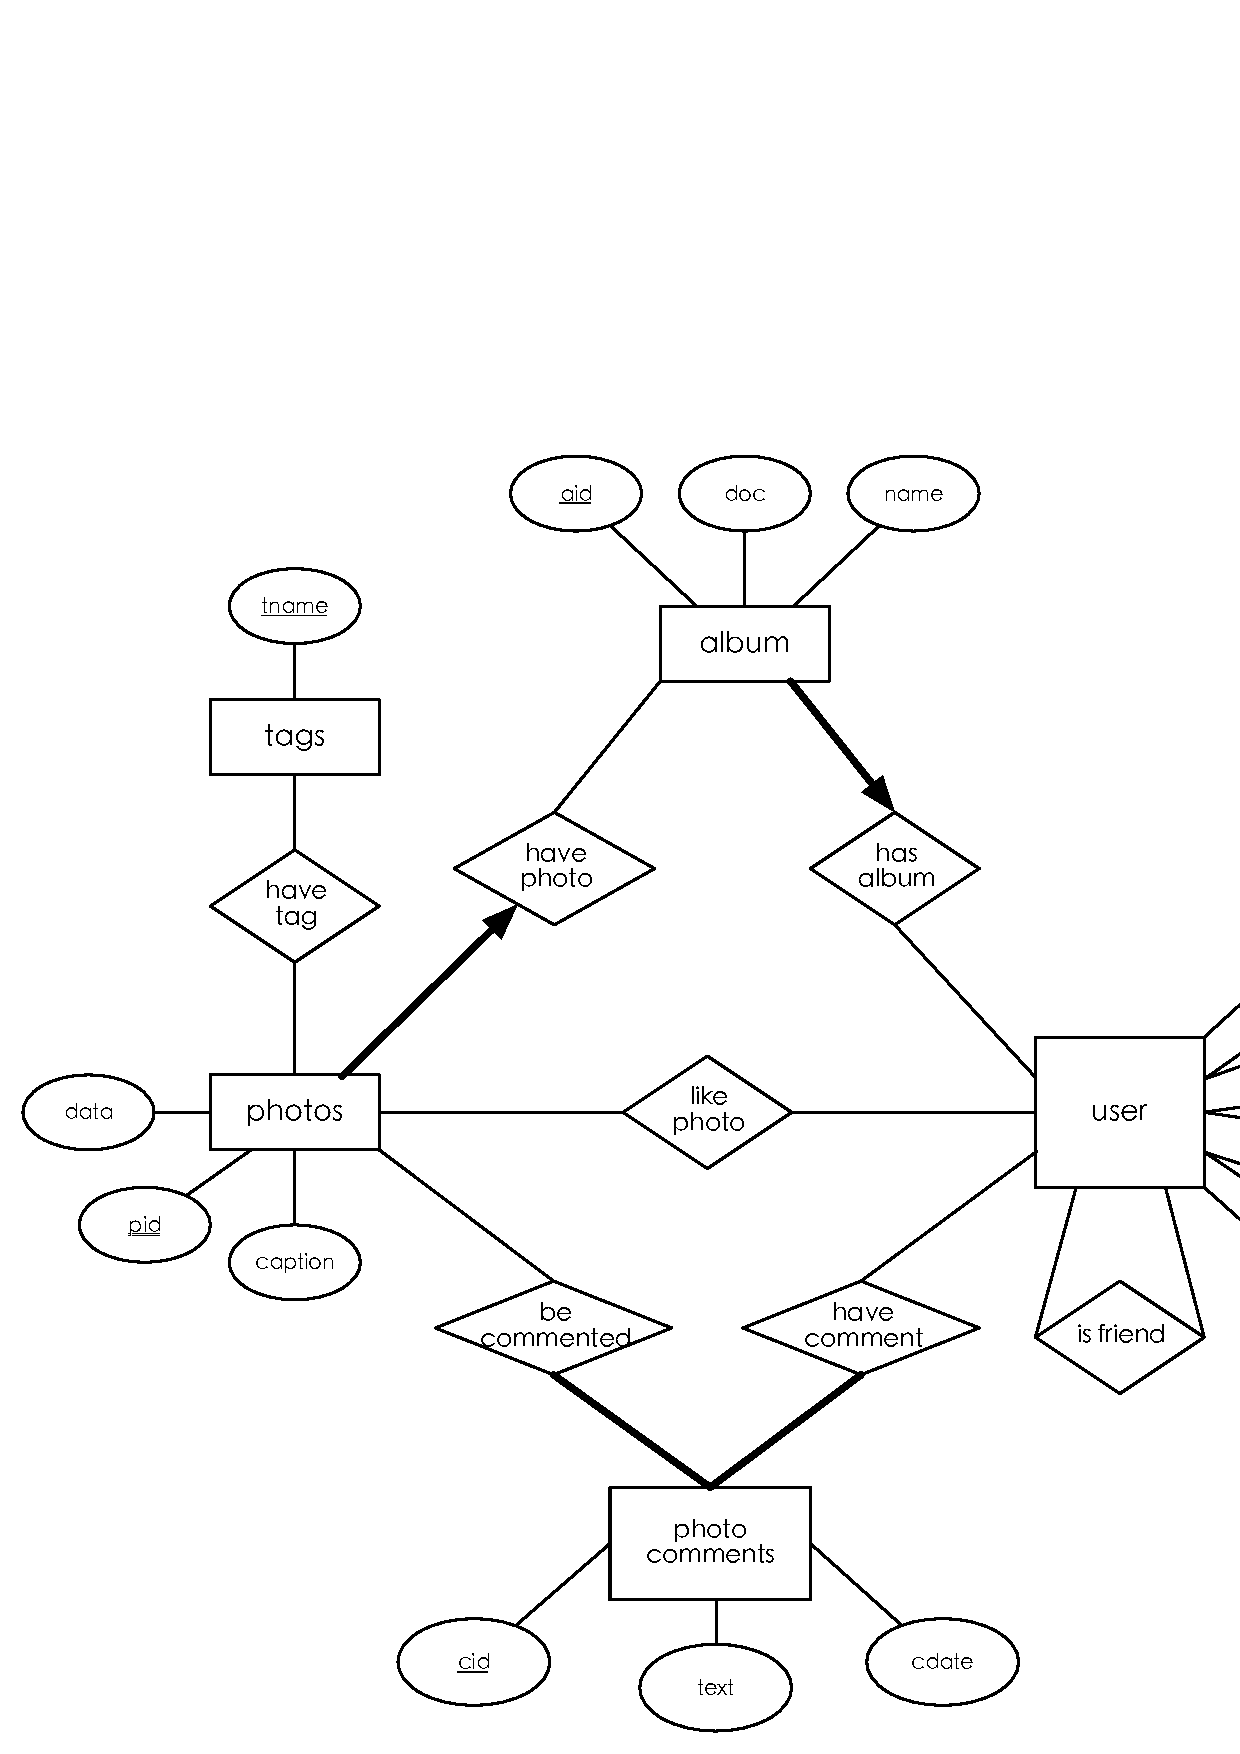
\includegraphics[width=6in]{pa1.png} 

\section{The Schema}
\begin{lstlisting}[frame=none]		 	% Start the code-block SQL

CREATE DATABASE photoshare;
USE photoshare;

CREATE TABLE Users(
   uid  INTEGER NOT NULL AUTO_INCREMENT,
   fname  VARCHAR(20) NOT NULL,
   lname  VARCHAR(20) NOT NULL,
   email  VARCHAR(50) UNIQUE,
   dob  DATE,
   hometown  VARCHAR(20),
   gender  CHAR(1),
   password  VARCHAR(20) NOT NULL,
   PRIMARY KEY  (uid)
   );

CREATE TABLE Albums(
   aid  INTEGER NOT NULL AUTO_INCREMENT,
   aname  VARCHAR(20) NOT NULL,
   doc  TIMESTAMP DEFAULT current_timestamp,
   uid INTEGER NOT NULL,
   PRIMARY KEY  (aid),
   FOREIGN KEY (uid) REFERENCES Users(uid)
  	ON DELETE CASCADE
   );
/* Assumption:
 each album has to belong to one user 
 includes album entity and 'own' relationship
*/

CREATE TABLE Photos(
   pid  INTEGER NOT NULL AUTO_INCREMENT,
   caption  VARCHAR(200),
   path VARCHAR(200) NOT NULL,
   aid INTEGER NOT NULL,
   PRIMARY KEY  (pid),
   FOREIGN KEY (aid) REFERENCES Albums(aid)
  	ON DELETE CASCADE
   );
/* Assumption:
  each photo has to belong to one album, 
  a photo copied from one album to another will have its 
  own (different) pid. */

CREATE TABLE Tags(
	 pid INTEGER NOT NULL,
	 tname VARCHAR(50) NOT NULL,
   PRIMARY KEY (pid, tname),
	 FOREIGN KEY (pid) REFERENCES Photos(pid) ON DELETE CASCADE
   );

CREATE TABLE isFriend(
   uid  INTEGER NOT NULL,
   fuid  INTEGER NOT NULL,
   PRIMARY KEY  (uid, fuid),
   FOREIGN KEY  (uid) REFERENCES Users(uid)
   	   ON DELETE CASCADE,
   FOREIGN KEY  (fuid) REFERENCES Users(uid)
   	   ON DELETE CASCADE,
   CHECK (uid <> fuid)
   );
/* Assumption: a user cannot be friend to him/herself;  
   (A,B) and (B,A) are different in this table */

CREATE TABLE Comments(
   cid  INTEGER NOT NULL AUTO_INCREMENT,
   cdate  TIMESTAMP DEFAULT current_timestamp,
   text  VARCHAR(255),
   pid  INTEGER NOT NULL,
   uid  INTEGER NOT NULL, 
   PRIMARY KEY  (cid),
   FOREIGN KEY  (pid) REFERENCES Photos(pid)
      ON DELETE CASCADE,
   FOREIGN KEY  (uid) REFERENCES Users(uid)
   );

CREATE TABLE likePhoto(
   uid  INTEGER,
   pid  INTEGER,
   PRIMARY KEY  (uid, pid),
   FOREIGN KEY  (uid) REFERENCES Users(uid)
   	   ON DELETE CASCADE,
   FOREIGN KEY  (pid) REFERENCES Photos(pid)
   	   ON DELETE CASCADE
   );

create view contribution as select up,fname,cc,cp,cc+cp from Users,
   (select uid as up, ifnull(count(pid),0) as cp from
      (select u.uid,p.pid from photos p RIGHT JOIN albums a ON a.aid = p.aid right join users u on u.uid=a.uid) b
      GROUP BY uid) a1,
   (select uid as uc,ifnull(count(cid),0) as cc from
      (select u.uid,c.cid from comments c RIGHT JOIN users u ON c.uid = u.uid) b group by uid) b1
   where uc=up and uc<>-1 and uc=uid
   order by cc+cp desc;

create view tagcount as
SELECT tname,count(tname) as ct
   from Tags
   group by tname
   ORDER BY ct desc;


INSERT INTO Users(uid,fname,lname,password) VALUES ('-1','guest','guest','password');
/* for unregistered users */

\end{lstlisting}


\section{The Constrains}
The entity set \textbf{Album} has a key constraint in the relationship set \textbf{hasAlbum}.\\
The entity set \textbf{Photos} has a key constraint in the relationship set \textbf{havePhoto}.

\end{document}  